\documentclass{book}
\usepackage[landscape,a3paper,left=0.5cm,right=1in,top=1in,bottom=1in]{geometry}
\usepackage{amsmath}
\usepackage{xcolor}
\usepackage{tikz}
\usepackage{pgfplots}
\usepackage{booktabs}
\usepackage{multirow}
\usepackage{amsmath,amssymb}

\begin{document}

\vspace{2cm}

\begin{center}\underline{\textsc{Equiv + Permut} for Test of 99 small instances of knapsack}
\vspace{0.5cm}

\begin{tabular}{cc} & no-solver\\\\\tikz{\node (a) at (0.0,4) {\textsc{Algo}};\node (a) at (0.0,0) {};} & 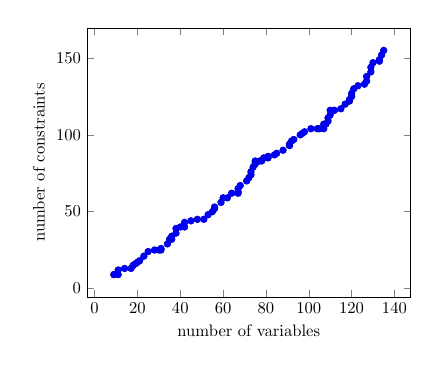
\begin{tikzpicture}[scale=0.6]
\begin{axis}[scatter, point meta=\thisrow{time}, only marks, colorbar, colorbar horizontal,colorbar style={ylabel={Time (min)}, ylabel style={rotate=270},}, colorbar to name={storedcolorbar1},, xlabel=number of variables,ylabel=number of constraints]

\addplot table[x=x,y=y]  { 
 x y time
 9 9 0.05 
 9 9 0.0 
 11 9 0.0 
 11 12 0.0 
 14 13 0.0 
 17 13 0.0 
 18 15 0.0 
 19 16 0.0 
 20 17 0.0 
 21 18 0.0 
 23 21 0.0 
 25 24 0.0 
 28 25 0.0 
 30 25 0.0 
 31 25 0.0 
 31 26 0.0 
 34 29 0.0 
 35 32 0.0 
 36 32 0.0 
 36 34 0.0 
 38 36 0.0 
 38 39 0.0 
 40 40 0.0 
 42 40 0.0 
 42 43 0.0 
 45 44 0.0 
 48 45 0.0 
 51 45 0.0 
 53 48 0.0 
 55 50 0.0 
 56 52 0.0 
 56 53 0.0 
 59 56 0.0 
 60 59 0.0 
 62 59 0.0 
 64 62 0.0 
 67 62 0.0 
 67 63 0.0 
 67 65 0.0 
 68 67 0.0 
 71 70 0.0 
 72 72 0.0 
 73 74 0.0 
 73 76 0.0 
 74 79 0.0 
 75 81 0.0 
 75 82 0.0 
 75 83 0.0 
 77 83 0.0 
 78 83 0.0 
 79 85 0.0 
 81 85 0.0 
 81 86 0.0 
 84 87 0.0 
 85 88 0.0 
 88 90 0.0 
 91 93 0.0 
 91 94 0.0 
 92 96 0.0 
 93 97 0.0 
 96 100 0.0 
 97 101 0.0 
 98 102 0.0 
 101 104 0.0 
 104 104 0.0 
 105 104 0.0 
 107 104 0.0 
 107 107 0.0 
 108 107 0.0 
 109 109 0.0 
 109 111 0.0 
 110 113 0.0 
 110 116 0.0 
 112 116 0.0 
 115 117 0.0 
 117 120 0.0 
 119 122 0.0 
 119 123 0.0 
 120 125 0.0 
 120 127 0.0 
 121 130 0.0 
 123 132 0.0 
 126 133 0.0 
 127 135 0.0 
 127 138 0.0 
 129 141 0.0 
 129 144 0.0 
 130 147 0.0 
 133 148 0.0 
 133 149 0.0 
 134 152 0.0 
 135 155 0.0 
};

\end{axis}
\end{tikzpicture}

\\
\tikz{\node (a) at (0.0,4) {\textsc{AlgoEnhanced}};\node (a) at (0.0,0) {};} & 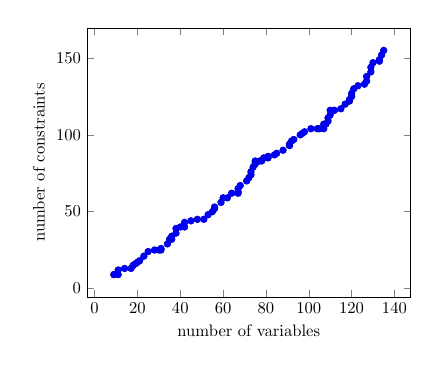
\begin{tikzpicture}[scale=0.6]
\begin{axis}[scatter, point meta=\thisrow{time}, only marks, , xlabel=number of variables,ylabel=number of constraints]

\addplot table[x=x,y=y]  { 
 x y time
 9 9 0.05 
 9 9 0.0 
 11 9 0.0 
 11 12 0.0 
 14 13 0.0 
 17 13 0.0 
 18 15 0.0 
 19 16 0.0 
 20 17 0.0 
 21 18 0.0 
 23 21 0.0 
 25 24 0.0 
 28 25 0.0 
 30 25 0.0 
 31 25 0.0 
 31 26 0.0 
 34 29 0.0 
 35 32 0.0 
 36 32 0.0 
 36 34 0.0 
 38 36 0.0 
 38 39 0.0 
 40 40 0.0 
 42 40 0.0 
 42 43 0.0 
 45 44 0.0 
 48 45 0.0 
 51 45 0.0 
 53 48 0.0 
 55 50 0.0 
 56 52 0.0 
 56 53 0.0 
 59 56 0.0 
 60 59 0.0 
 62 59 0.0 
 64 62 0.0 
 67 62 0.0 
 67 63 0.0 
 67 65 0.0 
 68 67 0.0 
 71 70 0.0 
 72 72 0.0 
 73 74 0.0 
 73 76 0.0 
 74 79 0.0 
 75 81 0.0 
 75 82 0.0 
 75 83 0.0 
 77 83 0.0 
 78 83 0.0 
 79 85 0.0 
 81 85 0.0 
 81 86 0.0 
 84 87 0.0 
 85 88 0.0 
 88 90 0.0 
 91 93 0.0 
 91 94 0.0 
 92 96 0.0 
 93 97 0.0 
 96 100 0.0 
 97 101 0.0 
 98 102 0.0 
 101 104 0.0 
 104 104 0.0 
 105 104 0.0 
 107 104 0.0 
 107 107 0.0 
 108 107 0.0 
 109 109 0.0 
 109 111 0.0 
 110 113 0.0 
 110 116 0.0 
 112 116 0.0 
 115 117 0.0 
 117 120 0.0 
 119 122 0.0 
 119 123 0.0 
 120 125 0.0 
 120 127 0.0 
 121 130 0.0 
 123 132 0.0 
 126 133 0.0 
 127 135 0.0 
 127 138 0.0 
 129 141 0.0 
 129 144 0.0 
 130 147 0.0 
 133 148 0.0 
 133 149 0.0 
 134 152 0.0 
 135 155 0.0 
};

\end{axis}
\end{tikzpicture}

\\
\\\\
\multicolumn{2}{c}{\ref{storedcolorbar1}}\end{tabular}\end{center}

\newpage

\begin{center}\underline{\textsc{Non-Equiv + Permut} for Test of 99 small instances of knapsack}
\vspace{0.5cm}

\begin{tabular}{cc} & no-solver\\\\\tikz{\node (a) at (0.0,4) {\textsc{Algo}};\node (a) at (0.0,0) {};} & 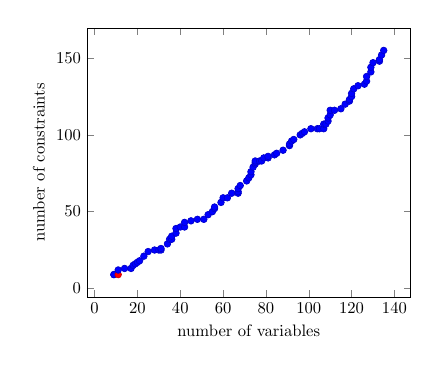
\begin{tikzpicture}[scale=0.6]
\begin{axis}[scatter, point meta=\thisrow{time}, only marks, colorbar, colorbar horizontal,colorbar style={ylabel={Time (min)}, ylabel style={rotate=270},}, colorbar to name={storedcolorbar2},, xlabel=number of variables,ylabel=number of constraints]

\addplot table[x=x,y=y]  { 
 x y time
 9 9 0.05 
 9 9 0.0 
 11 9 1440.0 
 11 12 0.0 
 14 13 0.0 
 17 13 0.0 
 18 15 0.0 
 19 16 0.0 
 20 17 0.0 
 21 18 0.0 
 23 21 0.0 
 25 24 0.0 
 28 25 0.0 
 30 25 0.0 
 31 25 0.0 
 31 26 0.0 
 34 29 0.0 
 35 32 0.0 
 36 32 0.0 
 36 34 0.0 
 38 36 0.0 
 38 39 0.0 
 40 40 0.0 
 42 40 0.0 
 42 43 0.0 
 45 44 0.0 
 48 45 0.0 
 51 45 0.0 
 53 48 0.0 
 55 50 0.0 
 56 52 0.0 
 56 53 0.0 
 59 56 0.0 
 60 59 0.0 
 62 59 0.0 
 64 62 0.0 
 67 62 0.0 
 67 63 0.0 
 67 65 0.0 
 68 67 0.0 
 71 70 0.0 
 72 72 0.0 
 73 74 0.0 
 73 76 0.0 
 74 79 0.0 
 75 81 0.0 
 75 82 0.0 
 75 83 0.0 
 77 83 0.0 
 78 83 0.0 
 79 85 0.0 
 81 85 0.0 
 81 86 0.0 
 84 87 0.0 
 85 88 0.0 
 88 90 0.0 
 91 93 0.0 
 91 94 0.0 
 92 96 0.0 
 93 97 0.0 
 96 100 0.0 
 97 101 0.0 
 98 102 0.0 
 101 104 0.0 
 104 104 0.0 
 105 104 0.0 
 107 104 0.0 
 107 107 0.0 
 108 107 0.0 
 109 109 0.0 
 109 111 0.0 
 110 113 0.0 
 110 116 0.0 
 112 116 0.0 
 115 117 0.0 
 117 120 0.0 
 119 122 0.0 
 119 123 0.0 
 120 125 0.0 
 120 127 0.0 
 121 130 0.0 
 123 132 0.0 
 126 133 0.0 
 127 135 0.0 
 127 138 0.0 
 129 141 0.0 
 129 144 0.0 
 130 147 0.0 
 133 148 0.0 
 133 149 0.0 
 134 152 0.0 
 135 155 0.0 
};

\end{axis}
\end{tikzpicture}

\\
\tikz{\node (a) at (0.0,4) {\textsc{AlgoEnhanced}};\node (a) at (0.0,0) {};} & 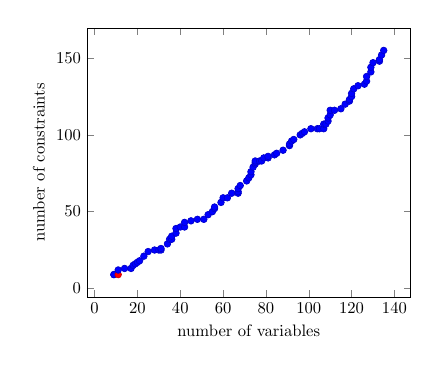
\begin{tikzpicture}[scale=0.6]
\begin{axis}[scatter, point meta=\thisrow{time}, only marks, , xlabel=number of variables,ylabel=number of constraints]

\addplot table[x=x,y=y]  { 
 x y time
 9 9 0.05 
 9 9 0.0 
 11 9 1440.0 
 11 12 0.0 
 14 13 0.0 
 17 13 0.0 
 18 15 0.0 
 19 16 0.0 
 20 17 0.0 
 21 18 0.0 
 23 21 0.0 
 25 24 0.0 
 28 25 0.0 
 30 25 0.0 
 31 25 0.0 
 31 26 0.0 
 34 29 0.0 
 35 32 0.0 
 36 32 0.0 
 36 34 0.0 
 38 36 0.0 
 38 39 0.0 
 40 40 0.0 
 42 40 0.0 
 42 43 0.0 
 45 44 0.0 
 48 45 0.0 
 51 45 0.0 
 53 48 0.0 
 55 50 0.0 
 56 52 0.0 
 56 53 0.0 
 59 56 0.0 
 60 59 0.0 
 62 59 0.0 
 64 62 0.0 
 67 62 0.0 
 67 63 0.0 
 67 65 0.0 
 68 67 0.0 
 71 70 0.0 
 72 72 0.0 
 73 74 0.0 
 73 76 0.0 
 74 79 0.0 
 75 81 0.0 
 75 82 0.0 
 75 83 0.0 
 77 83 0.0 
 78 83 0.0 
 79 85 0.0 
 81 85 0.0 
 81 86 0.0 
 84 87 0.0 
 85 88 0.0 
 88 90 0.0 
 91 93 0.0 
 91 94 0.0 
 92 96 0.0 
 93 97 0.0 
 96 100 0.0 
 97 101 0.0 
 98 102 0.0 
 101 104 0.0 
 104 104 0.0 
 105 104 0.0 
 107 104 0.0 
 107 107 0.0 
 108 107 0.0 
 109 109 0.0 
 109 111 0.0 
 110 113 0.0 
 110 116 0.0 
 112 116 0.0 
 115 117 0.0 
 117 120 0.0 
 119 122 0.0 
 119 123 0.0 
 120 125 0.0 
 120 127 0.0 
 121 130 0.0 
 123 132 0.0 
 126 133 0.0 
 127 135 0.0 
 127 138 0.0 
 129 141 0.0 
 129 144 0.0 
 130 147 0.0 
 133 148 0.0 
 133 149 0.0 
 134 152 0.0 
 135 155 0.0 
};

\end{axis}
\end{tikzpicture}

\\
\\\\
\multicolumn{2}{c}{\ref{storedcolorbar2}}\end{tabular}\end{center}

\newpage

\end{document}